\documentclass{article}
\usepackage[utf8]{inputenc}
\usepackage{amsmath}
\usepackage{mathtools}
\usepackage[a4paper,left=0.8in,right=0.8in,bottom=1in]{geometry}
\setlength{\parskip}{1em}
\setlength{\parindent}{0em}
\usepackage{floatrow}
\usepackage{graphicx}
\renewcommand{\familydefault}{\ttdefault}
\title{\huge\texttt{CS215 Assignment 3}}
\author{Aquib Nawaz(190050023),Rajesh Dasari(190050030),\\\texttt{Paavan Kumar(190050051)}}
\date{\texttt{27 September 2020}}

\begin{document}

\maketitle

\section* {Question 1}
\subsection* {a)}
The value of $X_1 = 1$,since the first color is always distinct\\
Suppose the required probability be $p$\\
For acheiving the event of $i^{th}$ disticnt color, suppose there are $(i-1)$ distinct colors already present\\
The next color that can be choosen must be from $(n+1-i)$ colors\\
$p = \frac{n+1-i}{n}$\\
\subsection* {b)}
Here $X_i$ is the number of additional steps for reaching a ith distinct color from $X^{(i-1)}$\\
Therefore if $i$th color is to come at $k$th step , then the remaining $(k-1)$ must come from $(i-1)$ colors\\
Therefore $P(X_i = k) = {(\frac{i-1}{n})}^{k-1}( \frac{n+1-i}{n}$)\\
this is equivalent to \\
$P(X_i = k) = {(1-p)}^{(k-1)}p$ where $p$ is same as defined in part a \\
The parameter of the geometric random variable is $p$ where $p =  \frac{n+1-i}{n} $
\subsection* {c)}
The expectation of a geometric random variable is given by\\
$E(X_i) = \sum_0^\infty kP(X_i = k) $\\
$E(X_i) = \sum_0^\infty k{(1-p)}^{(k-1)}p$\\
Consider the expression\\
$S = \sum_0^N k{(1-p)}^{(k-1)}p$\\
$S -(1-p)S = \sum_0^N k{(1-p)}^{(k-1)}p - \sum_0^N k{(1-p)}^{(k)}p$\\
$pS = \sum_0^{N-1} (1-p)^k p - N(1-p)^Np$\\
$S = \sum_0^{N-1} (1-p)^k -N(1-p)^N$\\
$\lim_{N \to \inf} N(1-p)^N = 0 $ and $\lim_{N\to\inf}\sum_0^{N-1}(1-p)^k = \frac{1}{1-(1-p)} = \frac{1}{p} $\\
Therefore $E(X_i) = \frac{1}{p} $\\
$E(X_i^2) = \sum_0^\infty k^2P(X_i = k) $\\
$E(X_i^2) = \sum_0^\infty k^2{(1-p)}^{(k-1)}p$\\
Consider the expression\\
$S' = \sum_0^N k{(1-p)}^{(k-1)}p$\\
$S' -(1-p)S' = \sum_0^N k^2{(1-p)}^{(k-1)}p - \sum_0^N k^2{(1-p)}^{(k)}p$\\
$pS' = \sum_0^{N-1} (2k-1)(1-p)^{k-1} p - N^2(1-p)^Np$\\
$pS' = 2pS - \sum_0^{N-1}(1-p)^kp - N^2(1-p)^Np$\\
$S' = 2S - \sum_0^{N-1}(1-p)^k -N^2(1-p)^N $\\
$\lim_{N \to \inf} N^2(1-p)^N = 0 $ and $\lim_{N\to\inf}\sum_0^{N-1}(1-p)^k = \frac{1}{1-(1-p)} = \frac{1}{p} $\\
$E(X_i^2) = 2\lim_{N \to \inf}S -\frac{1}{p} $\\
$E(X_i^2) = \frac{1}{p}$\\
$Var(X_i) = E(X_i^2) - E(X_i)^2$\\
$Var(X_i) = \frac{1}{p}-\frac{1}{p^2}$\\
$Var(X_i) = \frac{p-1}{p^2}$\par 
$E(X_i) = \frac{1}{p} $ and $Var(X_i) = \frac{1-p}{p^2}$
\subsection*{d)}
$E(X^{(n)}) = E(\sum_1^n X_i)$\\
$E(X^{(n)}) = \sum_1^n E(X_i) = \sum_1^n\frac{1}{p_i} $\\ 
$E(X^{(n)}) = \frac{\sum_1^n (n)}{n+1-i}$\\
$E(X^{(n)}) = n \sum_1^n\frac{1}{i}$\par 
$E(X^{(n)}) = n \sum_1^n\frac{1}{i}$
\subsection*{e)}
$Var(X^{(n)}) = Var(\sum_1^n X_i)$\\
Since these are iid random variables\\
$Var(X^{(n)}) = \sum_1^n Var(X_i) = \sum_1^n\frac{1-p_i}{p_i^2} $\\ 
$Var(X^{(n)}) = \sum_1^n \frac{n(i-1)}{(n+1-i)^2}$\\
$Var(X^{(n)}) \leq \sum_1^n\frac{n^2}{(n+1-i)^2}$ Since $i < n+1$\\ 
$Var(X^{(n)}) \leq \sum_1^n\frac{n^2}{i^2} \leq n^2\sum_1^{\infty} \frac{1}{n^2} $\par 
$Var(X^{(n)}) \leq n^2 \frac{\pi^2}{6}$
\subsection*{f)}
Since we know that $\log(n+1) < \sum_1^n \frac{1}{i} < \log n + 1$\\
Hence $n\log(n+1) < n\sum_1^n \frac{1}{i} < n\log n + n$\\
Therefore $n\log(n+1) < E(X_i) < n\log n + n$\\
These are graphically depicted in the figure below\\
f(n) therefore is $n\log n $\\
\ffigbox{\caption {Graph1}}
    {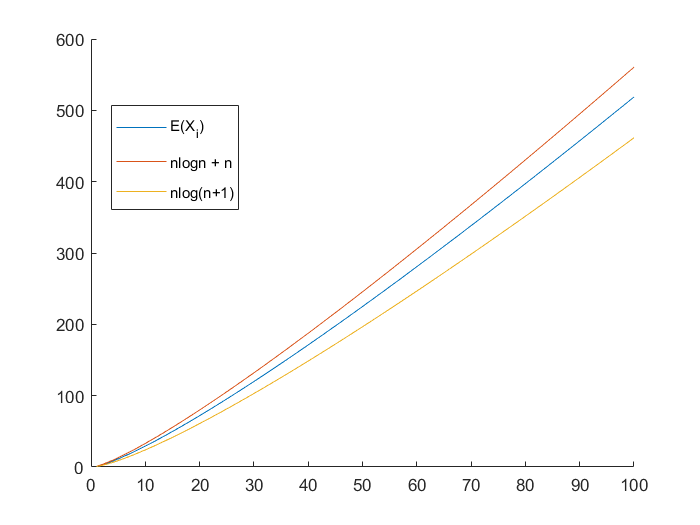
\includegraphics[width =9cm, height=7cm]{3q1.png}}
\section*{Question 2}
Since $F$ is a cumulative distribution function and it is given to be invertible which means the function has to be strictly increasing , because cdf is increasing and being invertible means $F(i)!=F(j)$ $ \forall \ i!=j$ , hence we can conclude $F $ is \textbf{strictly }increasing
\subsection*{a)}
Given invertible distribution function $F$ for a random variable.\\ Let the random variable generated by rand function is $u$.\\
Then we have to prove $v_{i} = F^{-1}(u_i)$ follows distribution $F$. where $u_i$ is generated from rand function.\\
To prove that it is enough to prove
 that $P|v_i\leq y| = F(y)$ for some y\\
Since distribution function is increasing as seen above\\
The solution sets, $v_i \leq y$ and $F(v_i) \leq F(y)$ are same ,Hence
\\ $P|v_i \leq y| = P|F(v_i) \leq F(y)| = P|u_i \leq F(y)|$\\
Also, $P|u_i \leq F(y)|=F(y)$ as $u_i$ is uniformly generated .\\
So, $P|v_i\leq y| = F(y)$

\subsection*{b)}
Here, $F_e(x) = \frac{\sum_{i=1}^n \textbf{1}(Y_i\leq x)}{n}$ and $D = max_x|F_e(x) - F(x)|$\\
Now $D = max_x|\frac{\sum_{i=1}^n \textbf{1}(Y_i\leq x)}{n} - F(x)| = max_{F(x)}|\frac{\sum_{i=1}^n \textbf{1}(F(Y_i)\leq F(x))}{n} - F(x)|$ as $F$ is increasing.\\
Replacing $F(x)$ by $y$ we can see that $D = E$ as   $0 \leq F(x) \leq 1$ and $F(Y_i) = U_i$\\
Since $Y_i = F^{-1}(U_i)$ from part a) because a distribution form $F$ can be witten in terms of a distribution from a \textbf{uniform} distribution\\
Hence there distribution function will be same or $P|D \leq d| = P|E \leq d|$\\
Now $P|D\geq d| = 1-P|D\leq d| = 1 - P|E \leq d| = P|E \geq d|$\\
Hence proved.\\
The practical significant of this result is that the error in generating random sample $v_i$ from inverse method is same as the error in getting  uniform distribution $u_i$. 

\section*{Question 3}
Since for both parts , the corruption value is from $\epsilon \sim\mathcal{N}(0,\sigma^2)$\\
We know that $f$ being the gaussian pdf , $f(\epsilon_i | \Theta) = \frac{1}{\sigma \sqrt{2\pi}}e^{-\frac{\epsilon_i^2}{2\sigma^2}}$\\
$f(\epsilon_1,\epsilon_2,....\epsilon_n | \Theta ) = \prod_1^n f(\epsilon_i | \Theta) $\\
$f(\epsilon_1,\epsilon_2,....\epsilon_n | \Theta ) = \prod_1^n \frac{1}{\sigma \sqrt{2\pi}}e^{-\frac{\epsilon_i^2}{2\sigma^2}} $
The log likelihood function hence is \\
$\mathcal{L}(\epsilon_1,\epsilon_2,....\epsilon_n | \Theta ) = \log f(\epsilon_1,\epsilon_2,....\epsilon_n | \Theta ) $\\
$\mathcal{L}(\epsilon_1,\epsilon_2,....\epsilon_n | \Theta ) = \sum_1^n \log(\frac{1}{\sigma \sqrt{2\pi}}e^{-\frac{\epsilon_i^2}{2\sigma^2}})$\\
$\mathcal{L}(\epsilon_1,\epsilon_2,....\epsilon_n | \Theta ) = \sum_1^n (-\frac{\epsilon_i^2}{2\sigma^2}- \log(\sigma \sqrt{2\pi}))$\\
$\mathcal{L}(\epsilon_1,\epsilon_2,....\epsilon_n | \Theta ) = \sum_1^n (-\frac{\epsilon_i^2}{2\sigma^2}) - n\log(\sigma \sqrt{2\pi})$\\
\vspace{-20pt}
\subsection*{a)}
\vspace{-10pt}
Maximum Likelihood based Plane fitting\\
Given that $Z$ is corrupted with values from a Gaussian distribution and the values of $X $ and $Y$ are known without any error\\
Consider the random variable $\epsilon$ where $\epsilon_i = Z_i - aX_i - bY_i - c$\\
Since the corrupted values are from a Gaussian $\epsilon \sim \mathcal{N}(0,\sigma^2)$\\
For the parameters $a,b,c$ and iid variables $\epsilon_i$, the maximum likelihood function is given by,\\
$G(a,b,c|\epsilon_1,\epsilon_2,....\epsilon_n) = f(\epsilon_1,\epsilon_2,....\epsilon_n | \Theta )$ where $\Theta = \{{a,b,c}\}$\\
since $\epsilon_i = Z_i - aX_i - bY_i - c$ , we have $\frac{\partial {\epsilon_i}}{\partial a} = -X_i$, $\frac{\partial {\epsilon_i}}{\partial b} = -Y_i$ and $\frac{\partial {\epsilon_i}}{\partial c} = -1$\\
differentiating w.r.t $a$ and equating to zero ,\\
$\frac{\partial \mathcal{L}(\epsilon_1,\epsilon_2,....\epsilon_n | \Theta )}{\partial a} = \sum_1^n \frac{\partial (-\frac{\epsilon_i^2}{2\sigma^2})}{\partial a}$\\
$\frac{-1}{2\sigma^2} \sum_1^n 2\epsilon_i \frac{\partial {\epsilon_i}}{\partial a} = 0$\par 
$\implies \sum_1^n \epsilon_iX_i = 0$\\ 
Similarly  differentiating w.r.t $b,c$ we get \\
$\sum_1^n \epsilon_iY_i = 0$ and $\sum_1^n \epsilon_i = 0$\\
writing these in equation form, we get \\
\begin{equation}
a \sum_1^n X_i^2 + b \sum_1^n X_iY_i + c \sum_1^n X_i = \sum X_iZ_i
\end{equation}
\begin{equation}
a \sum_1^n X_iY_i + b \sum_1^n Y_i^2 + c \sum_1^n Y_i = \sum Y_iZ_i
\end{equation}
\begin{equation}
a \sum_1^n X_i + b \sum_1^n Y_i + c \sum_1^n 1 = \sum Z_i
\end{equation}
In matrix form \\
\begin{gather} 
    \begin{bmatrix}
        \sum X_i^2 & \sum X_iY_i & \sum X_i \\
        \sum X_iY_i & \sum Y_i^2 & \sum Y_i\\
        \sum X_i & \sum Y_i & n
    \end{bmatrix}
    \begin{bmatrix}
    $a$ \\ $b$ \\$c$
    \end{bmatrix}
    =
    \begin{bmatrix}
    \sum X_iZ_i\\
    \sum Y_iZ_i\\
    \sum Z_i
    \end{bmatrix}
    \end{gather}
In Vector form \\
\begin{gather} 
    a
    \begin{bmatrix}
        \sum X_i^2 \\
        \sum X_iY_i\\
        \sum X_i
    \end{bmatrix}
    +
    b 
    \begin{bmatrix}
        \sum X_iY_i \\
        \sum Y_i^2\\
        \sum Y_i
    \end{bmatrix}
    +
    c
    \begin{bmatrix}
        \sum X_i \\
        \sum Y_i\\
        n 
    \end{bmatrix}
    =
    \begin{bmatrix}
    \sum X_iZ_i\\
    \sum Y_iZ_i\\
    \sum Z_i
    \end{bmatrix}
    \end{gather}
\subsection*{b)}
Given that $Z$ is corrupted with values from a Gaussian distribution and the values of $X $ and $Y$ are known without any error\\
Consider the random variable $\epsilon$ where $\epsilon_i = Z_i - a_1X_i^2 - a_2Y_i^2 - a_3X_iY_i - a_4X_i -a_5Y_i -a_6$\\
Since the corrupted values are from a Gaussian $\epsilon \sim \mathcal{N}(0,\sigma^2)$\\
For the parameters $a_1,a_2,a_3,a_4,a_5,a_6$ and iid variables $\epsilon_i$,\\ the maximum likelihood function is given by,\\
$G(a_1,a_2,a_3,a_4,a_5,a_6|\epsilon_1,\epsilon_2,....\epsilon_n) = f(\epsilon_1,\epsilon_2,....\epsilon_n | \Theta )$ where $\Theta = \{{a_1,a_2,a_3,a_4,a_5,a_6}\}$\\
since $\epsilon_i =  Z_i - a_1X_i^2 - a_2Y_i^2 - a_3X_iY_i - a_4X_i -a_5Y_i -a_6$ ,\\ we have $\frac{\partial {\epsilon_i}}{\partial a_1} = -X_i^2$, $\frac{\partial {\epsilon_i}}{\partial a_2} = -Y_i^2$, $\frac{\partial {\epsilon_i}}{\partial a_3} = -X_iY_i $, $\frac{\partial {\epsilon_i}}{\partial a_4} = -X_i $, $\frac{\partial {\epsilon_i}}{\partial a_5} = -Y_i $, $\frac{\partial {\epsilon_i}}{\partial a_6} = -1 $\\
differentiating w.r.t $a_i$ and equating to zero ,\\
$\frac{\partial \mathcal{L}(\epsilon_1,\epsilon_2,....\epsilon_n | \Theta )}{\partial a_i} = \sum_1^n \frac{\partial (-\frac{\epsilon_i^2}{2\sigma^2})}{\partial a_i}$\\
$\frac{-1}{2\sigma^2} \sum_1^n 2\epsilon_i \frac{\partial {\epsilon_i}}{\partial a_i} = 0$\par 
$\sum_1^n \epsilon_i \frac{\partial {\epsilon_i}}{\partial a_i} = 0$\par 
Hence the equations are\par 
$\sum_1^n \epsilon_i X_i^2 =0$, $\sum_1^n \epsilon_i Y_i^2 =0$, $\sum_1^n \epsilon_i X_iY_i =0$, $\sum_1^n \epsilon_i X_i =0$, $\sum_1^n \epsilon_i X_i =0$, and  $\sum_1^n \epsilon_i =0$
writing these in equation form using $\epsilon_i = Z_i - a_1X_i^2 - a_2Y_i^2 - a_3X_iY_i - a_4X_i -a_5Y_i -a_6$\\
\begin{equation}
a_1 \sum_1^n X_i^4 + a_2 \sum_1^n X_i^2Y_i^2 + a_3 \sum_1^n X_i^3Y_i + a_4 \sum_1^n X_i^3 +a_5 \sum_1^n X_i^2Y_i + a_6 \sum_1^n X_i^2= \sum X_i^2Z_i
\end{equation}
\begin{equation}
a_1 \sum_1^n X_i^2Y_i^2 + a_2 \sum_1^n Y_i^4 + a_3 \sum_1^n X_iY_i^3 + a_4 \sum_1^n X_iY_i^2 +a_5 \sum_1^n Y_i^3 + a_6 \sum_1^n Y_i^2= \sum Y_i^2Z_i
\end{equation}
\begin{equation}
a_1 \sum_1^n X_i^3Y_i + a_2 \sum_1^n X_iY_i^3 + a_3 \sum_1^n X_i^2Y_i^2 + + a_4 \sum_1^n X_i^2Y_i +a_5 \sum_1^n X_iY_i^2 + a_6 \sum_1^n X_iY_i = \sum X_iY_iZ_i
\end{equation}
\begin{equation}
a_1 \sum_1^n X_i^3 + a_2 \sum_1^n X_iY_i^2 + a_3 \sum_1^n X_i^2Y_i + a_4 \sum_1^n X_i^2 +a_5 \sum_1^n X_iY_i + a_6 \sum_1^n X_i = \sum X_iZ_i
\end{equation}
\begin{equation}
a_1 \sum_1^n X_i^2Y_i + a_2 \sum_1^n Y_i^3 + a_3 \sum_1^n X_iY_i^2 + a_4 \sum_1^n X_iY_i +a_5 \sum_1^n Y_i^2 + a_6 \sum_1^n Y_i = \sum Y_iZ_i
\end{equation}
\begin{equation}
a_1 \sum_1^n X_i^2 + a_2 \sum_1^n Y_i^2 + a_3 \sum_1^n X_iY_i + a_4 \sum_1^n X_i +a_5 \sum_1^n Y_i + a_6 \sum_1^n 1 = \sum Z_i
\end{equation}
In matrix form \\
\begin{gather} 
    \begin{bmatrix}
        \sum X_i^4 & \sum X_i^2Y_i^2 & \sum X_i^3Y_i & \sum X_i^3 & \sum X_i^2Y_i & \sum X_i^2 \\
        \sum X_i^2Y_i^2 & \sum Y_i^4 & \sum X_iY_i^3 & \sum X_iY_i^2 & \sum Y_i^3 & \sum Y_i^2 \\
        \sum X_i^3Y_i & \sum X_iY_i^3 & \sum X_i^2Y_i^2 & \sum X_i^2Y_i & \sum X_iY_i^2 & \sum X_iY_i \\
        \sum X_i^3 & \sum X_iY_i^2 & \sum X_i^2Y_i & \sum X_i^2 & \sum X_iY_i & \sum X_i \\
        \sum X_i^2Y_i & \sum Y_i^3 & \sum X_iY_i^2 & \sum X_iY_i & \sum Y_i^2 & \sum Y_i \\
        \sum X_i^2 & \sum Y_i^2 & \sum X_iY_i & \sum X_i & \sum Y_i & n
    \end{bmatrix}
    \begin{bmatrix}
    a_1 \\ a_2 \\a_3 \\ a_4 \\ a_5 \\ a_6
    \end{bmatrix}
    =
    \begin{bmatrix}
    \sum X_i^2Z_i\\
    \sum Y_i^2Z_i\\
    \sum X_iY_iZ_i\\
    \sum X_iZ_i\\
    \sum Y_iZ_i\\
    \sum Z_i
    \end{bmatrix}
    \end{gather}
In vector form,\\
\begin{gather} 
    a_1
    \begin{bmatrix}
        \sum X_i^4\\
        \sum X_i^2Y_i^2\\
        \sum X_i^3Y_i\\
        \sum X_i^3\\
        \sum X_i^2Y_i\\
        \sum X_i^2
    \end{bmatrix}
    +
    a_2 
    \begin{bmatrix}
        \sum X_i^2Y_i^2\\
        \sum Y_i^4\\
        \sum X_iY_i^3\\
        \sum X_iY_i^2\\
        \sum Y_i^3\\
        \sum Y_i^2
    \end{bmatrix}
    +
    a_3
    \begin{bmatrix}
        \sum X_i^3Y_i\\
        \sum X_iY_i^3\\
        \sum X_i^2Y_i^2\\
        \sum X_i^2Y_i\\
        \sum X_iY_i^2\\
        \sum X_iY_i
    \end{bmatrix}
    +
    a_4
    \begin{bmatrix}
    \sum X_i^3\\
    \sum X_iY_i^2\\
    \sum X_i^2Y_i\\
    \sum X_i^2\\
    \sum X_iY_i\\
    \sum X_i
    \end{bmatrix}
    +
    a_5
    \begin{bmatrix}
    \sum X_i^2Y_i\\
    \sum Y_i^3\\
    \sum X_iY_i^2\\
    \sum X_iY_i\\
    \sum Y_i^2\\
    \sum X_i
    \end{bmatrix}
    +
    a_6
    \begin{bmatrix}
    \sum X_i^2\\
    \sum Y_i^2\\
    \sum X_iY_i\\
    \sum X_i\\
    \sum Y_i\\
     n
    \end{bmatrix}
    =
    \begin{bmatrix}
    \sum X_i^2Z_i\\
    \sum Y_i^2Z_i\\
    \sum X_iY_iZ_i\\
    \sum X_iZ_i\\
    \sum Y_iZ_i\\
    \sum Z_i
    \end{bmatrix}
    \end{gather}
\subsection*{c)}
The code for this part is attached with the name \textsf{\textbf{{\sf A3q3.m}}}\\
The code upon execution gives four values a, b, c and std\_dev as the outputs\\
The value of parameters for the given text file \\
a = 10.0022\\
b = 19.9980\\
c = 29.9516\\
and \\
$\sigma $ = 4.8030 \\
The predicted equation of the plane is $Z = 10.0022X+19.9980Y+29.9516$
\section*{Question 4}
\subsection*{b)}
The joint likelihood of the samples in $V$ determined from the estimate pdf built from samples in $T$ by Kernel density estimation is\\
$\mathcal{L} = \prod_{y_i \in V} \hat{p_n}(y_i;\sigma) = \prod_{y_i \in V}\dfrac{\sum_{x_j \in T} \exp{(-(y_i - x_j)^2/(2 \sigma^2))}}{n \sigma \sqrt{2 \pi}}$\\
Where $x_j$ is from $T$ and $n = 750 $ (this case)
\subsection*{c) d)}
The code for this part is included with the name \textbf{Aq4.m}\\
The code upon execution gives the values of $\sigma$ for part c and part d as the output\\
And it produces four graphs,figure1 and figure2 for part c, and figure3 and figure4 for part d\\
Note: for some random distributions generated the value of $LL$ at $\sigma = 0.001$ shoots down to $-inf$\\
FOR PART C\\
The value of $\sigma_1$ that yielded the best value of LL is 1 \\
(note that this quantity may change with the value of sample size and this is a small sample space)\\
For this sigma the plot for x = [-8:0.1:8] is overlaid with true density and is enclosed\\
The value of $\sigma_2$ that yields the best value of D must be around $\sigma$ since the plot mentioned above is very much close to the true sigma value and hence plotting the D versus $\log \sigma$ for $\sigma$ between $\sigma_1e^{-1}$ and $\sigma_1e$\\
The value of $\sigma_2$ that yields the best value for this particular case is 1.5984\\
For this $\sigma_2$, the plot of $\hat{p_n}(x_i;\sigma)$ is overlaid with that of true density and that for $\sigma_1$
\begin{figure}[H]
    \begin{floatrow}
    \ffigbox{\caption {LL versus $\log \sigma$}}
    {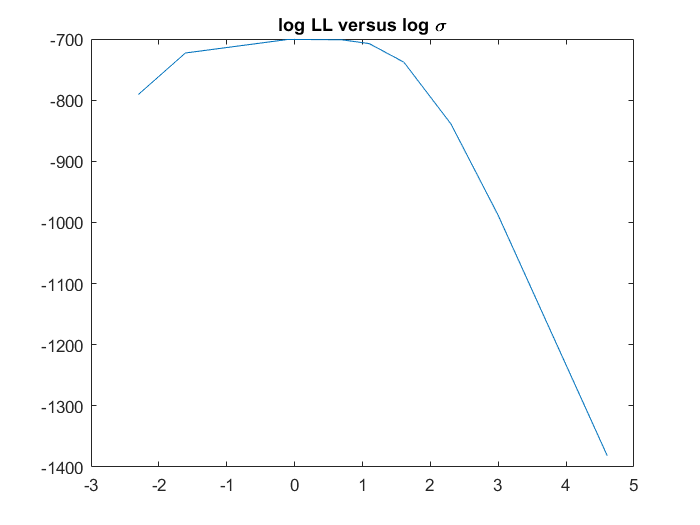
\includegraphics[width =9.2cm, height=8cm]{logll.png}}
    \ffigbox{\caption {Kernel and true Densities for $\sigma_1$}}
    {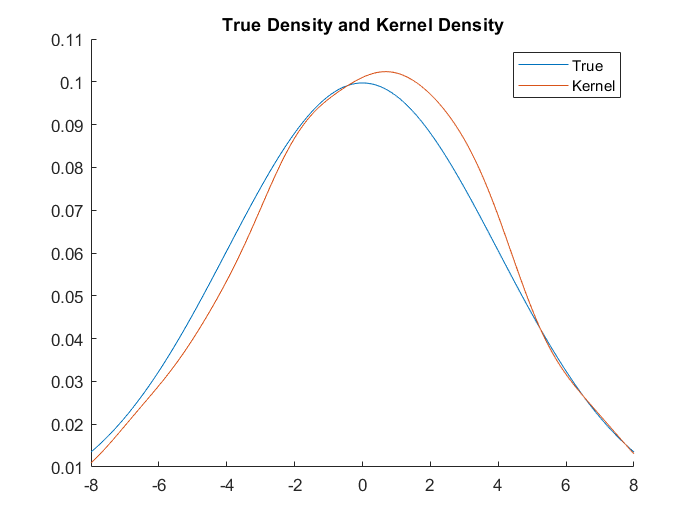
\includegraphics[width =9.2cm, height=8cm]{kernel1.png}}
    \end{floatrow}
    \begin{floatrow}
    \ffigbox{\caption {D versus $\log \sigma$ around $\sigma_1$}}
    {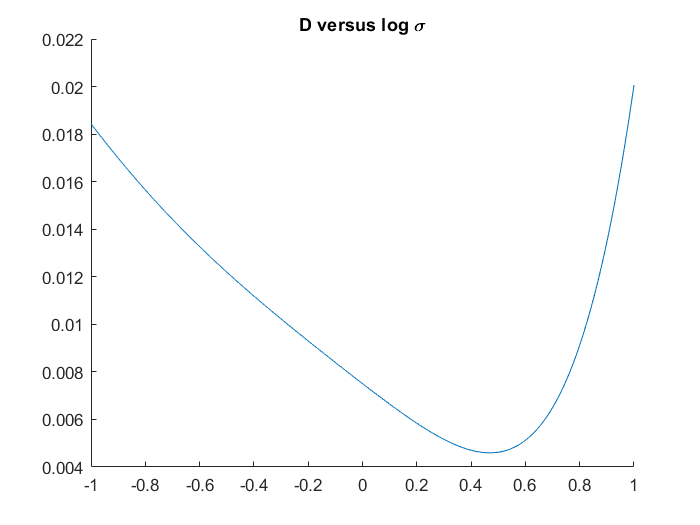
\includegraphics[width =9.2cm, height=9cm]{Dlog.png}}
    \ffigbox{\caption {Kernel and true densities for $\sigma_2$(final) along with $\sigma_1$(approx) overlaid}}
    {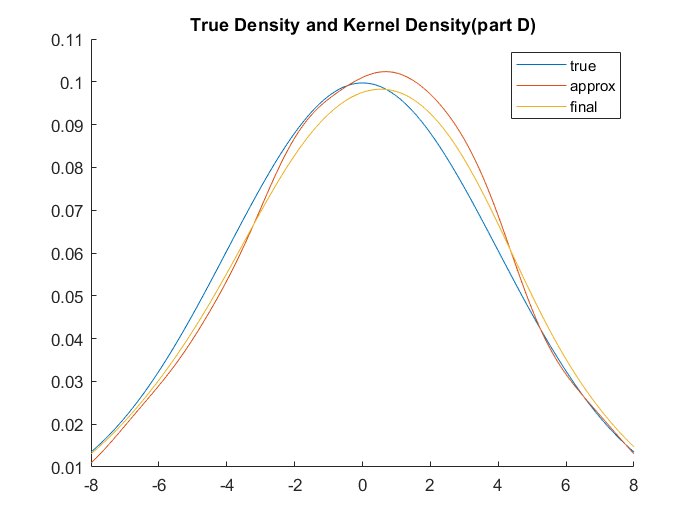
\includegraphics[width =9.2cm, height=9cm]{final.png}}
    \end{floatrow}
    \end{figure}
\subsection*{e)}
If V and T were same , we would be applying the maximum likelihood estimation(MLE) for T w.r.t to the estimated pdf of T by Kernel density estimation,The LL of T w.rt T doesnt have a maximum and approaches $\infty$ as $\sigma \to 0$ which would mean $\sigma = 0$ is the parameter at LL is maximised , but technically $\sigma \neq 0$\newpage
This is due to fact that $\forall \ x\  \exists \ k < 750$ , the value of $x-x_k=0$ since $V=T$,\\ which means for $i=k, \ \exp{(-(x - x_i)^2/(2 \sigma^2))}= 1$ for all $\sigma$ \\And for $i\ !=k, \ \exp{(-(x - x_i)^2/(2 \sigma^2))} = 0 $ as $\sigma \to 0$\\
Hence as $\sigma \to 0$ , $\hat{p_n}(x,\sigma) = \lambda(\frac{1}{\sigma}) \to \infty$\\
$\implies LL\to \infty$, Hence no maximum likelihood for this LL.\\
Hence cross validation procedure fails and gives wrong values for $\sigma$ as the maximum value of LL occurs at a palce where $\sigma$ is not defined.\\
\end{document}